%% Преамбула TeX-файла

% 1. Стиль и язык
\documentclass[utf8x, times, 14pt]{G7-32} % Стиль (по умолчанию будет 14pt)
\bibliographystyle{gost780u}

% Остальные стандартные настройки убраны в preamble.inc.tex.
\sloppy

% Настройки стиля ГОСТ 7-32
% Для начала определяем, хотим мы или нет, чтобы рисунки и таблицы нумеровались в пределах раздела, или нам нужна сквозная нумерация.
\EqInChapter % формулы будут нумероваться в пределах раздела
\TableInChapter % таблицы будут нумероваться в пределах раздела
\PicInChapter % рисунки будут нумероваться в пределах раздела

% Добавляем гипертекстовое оглавление в PDF
\usepackage[
bookmarks=true, colorlinks=true, unicode=true,
urlcolor=black,linkcolor=black, anchorcolor=black,
citecolor=black, menucolor=black, filecolor=black,
]{hyperref}

\AfterHyperrefFix

\usepackage{microtype}% полезный пакет для микротипографии, увы под xelatex мало чего умеет, но под pdflatex хорошо улучшает читаемость

% Тире могут быть невидимы в Adobe Reader
\ifInvisibleDashes
\MakeDashesBold
\fi


\usepackage{graphicx}   % Пакет для включения рисунков

% С такими оно полями оно работает по-умолчанию:
% \RequirePackage[left=20mm,right=10mm,top=20mm,bottom=20mm,headsep=0pt,includefoot]{geometry}
% Если вас тошнит от поля в 10мм --- увеличивайте до 20-ти, ну и про переплёт не забывайте:
\geometry{right=20mm}
\geometry{left=30mm}
\geometry{bottom=20mm}
\geometry{ignorefoot}% считать от нижней границы текста

\usepackage{rotating}

% доп. позиционирование таблиц
\usepackage{float}

% таблицы с автоматическим определением ширины
\usepackage{tabularx}

% Пакет Tikz
\usepackage{tikz}
\usetikzlibrary{arrows,positioning,shadows}

% Произвольная нумерация списков.
\usepackage{enumerate}

% ячейки в несколько строчек
\usepackage{multirow}

% itemize внутри tabular
\usepackage{paralist,array}
\newcolumntype{Y}{>{\centering\arraybackslash}X}

%\setlength{\parskip}{1ex plus0.5ex minus0.5ex} % разрыв между абзацами
\setlength{\parskip}{1ex} % разрыв между абзацами
\usepackage{blindtext}

% Центрирование подписей к плавающим окружениям
%\usepackage[justification=centering]{caption}

\usepackage{newfloat}
\DeclareFloatingEnvironment[
placement={!ht},
name=Equation
]{eqndescNoIndent}
\edef\fixEqndesc{\noexpand\setlength{\noexpand\parindent}{\the\parindent}\noexpand\setlength{\noexpand\parskip}{\the\parskip}}
\newenvironment{eqndesc}[1][!ht]{%
    \begin{eqndescNoIndent}[#1]%
\fixEqndesc%
}
{\end{eqndescNoIndent}}
\usepackage{mathtext}

% Настройки листингов.
\ifPDFTeX
% 8 Листинги

\usepackage{listings}

% Значения по умолчанию
\lstset{
  basicstyle= \footnotesize,
  breakatwhitespace=true,% разрыв строк только на whitespacce
  breaklines=true,       % переносить длинные строки
%   captionpos=b,          % подписи снизу -- вроде не надо
  inputencoding=koi8-r,
  numbers=left,          % нумерация слева
  numberstyle=\footnotesize,
  showspaces=false,      % показывать пробелы подчеркиваниями -- идиотизм 70-х годов
  showstringspaces=false,
  showtabs=false,        % и табы тоже
  stepnumber=1,
  tabsize=4,              % кому нужны табы по 8 символов?
  frame=single
}

% Стиль для псевдокода: строчки обычно короткие, поэтому размер шрифта побольше
\lstdefinestyle{pseudocode}{
  basicstyle=\small,
  keywordstyle=\color{black}\bfseries\underbar,
  language=Pseudocode,
  numberstyle=\footnotesize,
  commentstyle=\footnotesize\it
}

% Стиль для обычного кода: маленький шрифт
\lstdefinestyle{realcode}{
  basicstyle=\scriptsize,
  numberstyle=\footnotesize
}

% Стиль для коротких кусков обычного кода: средний шрифт
\lstdefinestyle{simplecode}{
  basicstyle=\footnotesize,
  numberstyle=\footnotesize
}

% Стиль для BNF
\lstdefinestyle{grammar}{
  basicstyle=\footnotesize,
  numberstyle=\footnotesize,
  stringstyle=\bfseries\ttfamily,
  language=BNF
}

% Определим свой язык для написания псевдокодов на основе Python
\lstdefinelanguage[]{Pseudocode}[]{Python}{
  morekeywords={each,empty,wait,do},% ключевые слова добавлять сюда
  morecomment=[s]{\{}{\}},% комменты {а-ля Pascal} смотрятся нагляднее
  literate=% а сюда добавлять операторы, которые хотите отображать как мат. символы
    {->}{\ensuremath{$\rightarrow$}~}2%
    {<-}{\ensuremath{$\leftarrow$}~}2%
    {:=}{\ensuremath{$\leftarrow$}~}2%
    {<--}{\ensuremath{$\Longleftarrow$}~}2%
}[keywords,comments]

% Свой язык для задания грамматик в BNF
\lstdefinelanguage[]{BNF}[]{}{
  morekeywords={},
  morecomment=[s]{@}{@},
  morestring=[b]",%
  literate=%
    {->}{\ensuremath{$\rightarrow$}~}2%
    {*}{\ensuremath{$^*$}~}2%
    {+}{\ensuremath{$^+$}~}2%
    {|}{\ensuremath{$|$}~}2%
}[keywords,comments,strings]

% Подписи к листингам на русском языке.
\renewcommand\lstlistingname{Листинг}
\renewcommand\lstlistlistingname{Листинги}

\else
\usepackage{local-minted}
\fi

% Полезные макросы листингов.
% Любимые команды
\newcommand{\Code}[1]{\textbf{#1}}


% Стиль титульного листа и заголовки
%\include{00-title}


\begin{document}

\frontmatter % выключает нумерацию ВСЕГО; здесь начинаются ненумерованные главы: реферат, введение, глоссарий, сокращения и прочее.

\maketitle %создает титульную страницу


%\begin{executors}
%\personalSignature{Первый исполнитель}{ФИО}
%
%\personalSignature{Второй исполнитель}{ФИО}
%\end{executors}


%\listoffigures                         % Список рисунков

%\listoftables                          % Список таблиц

%\NormRefs % Нормативные ссылки 
% Команды \breakingbeforechapters и \nonbreakingbeforechapters
% управляют разрывом страницы перед главами.
% По-умолчанию страница разрывается.

% \nobreakingbeforechapters
% \breakingbeforechapters

%% Также можно использовать \Referat, как в оригинале
\begin{abstract}

   Для электрической сети, схема которой показана на *, на основании исходных данных по узлам и ветвям, приведенных в табл. * и *:
   
   \begin{enumerate}[1.]
   	\item Составить схему замещения сети и определить ее параметры
   	\item Выполнить расчеты потокораспределения и напряжений в узлах сети в нормальном режиме наибольших нагрузок.
   	\item Выполнить расчеты потокораспределения и напряжений в узлах сети в нормальном режиме наименьших нагрузок.
   	\item Выполнить расчеты потокораспределения и напряжений в узлах сети в послеаварийном
   	режиме (отключение одной цепи линии).
   	\item Оценить достаточность регулировочных диапазонов устройств РПН трансформаторов на
   	подстанции.
   	\item Рассчитать потери активной мощности и годовые потери электроэнергии в сети.
   \end{enumerate}

\end{abstract}

%%% Local Variables: 
%%% mode: latex
%%% TeX-master: "rpz"
%%% End: 


\tableofcontents

%\printnomenclature % Автоматический список сокращений

\Introduction

Целью выполнения расчетного задания является получение практических навыков по решению задач, связанных с составлением схем замещения основных элементов электрических сетей, к которым относятся линии электропередачи (ЛЭП) и подстанции (ПС), а также расчетам установившихся нормальных и послеаварийных режимов электрической сети и анализу полученных результатов.

Кроме того, в рамках расчетного задания решаются задачи оценки достаточности регулировочных диапазонов устройств регулирования напряжения трансформаторов на понижающей подстанции в различных режимах работы электрической сети, рассчитываются потери активной мощности и годовые потери электроэнергии в сети.

Полученные практические навыки необходимы для выполнения предстоящего курсового проекта по дисциплине «Электроэнергетические системы и сети» и будут полезны при подготовке выпускной квалификационной работы бакалавра.


\chapter{Исходные данные}
\label{cha:data}

Источником питания (ИП) электрической сети (рис.~\ref{fig:scheme}) является районная подстанция, работающая в составе электроэнергетической системы, с распределительными устройствами 110 и 220 кВ.

\renewcommand{\thefigure}{1}
\begin{figure}
	\centering
	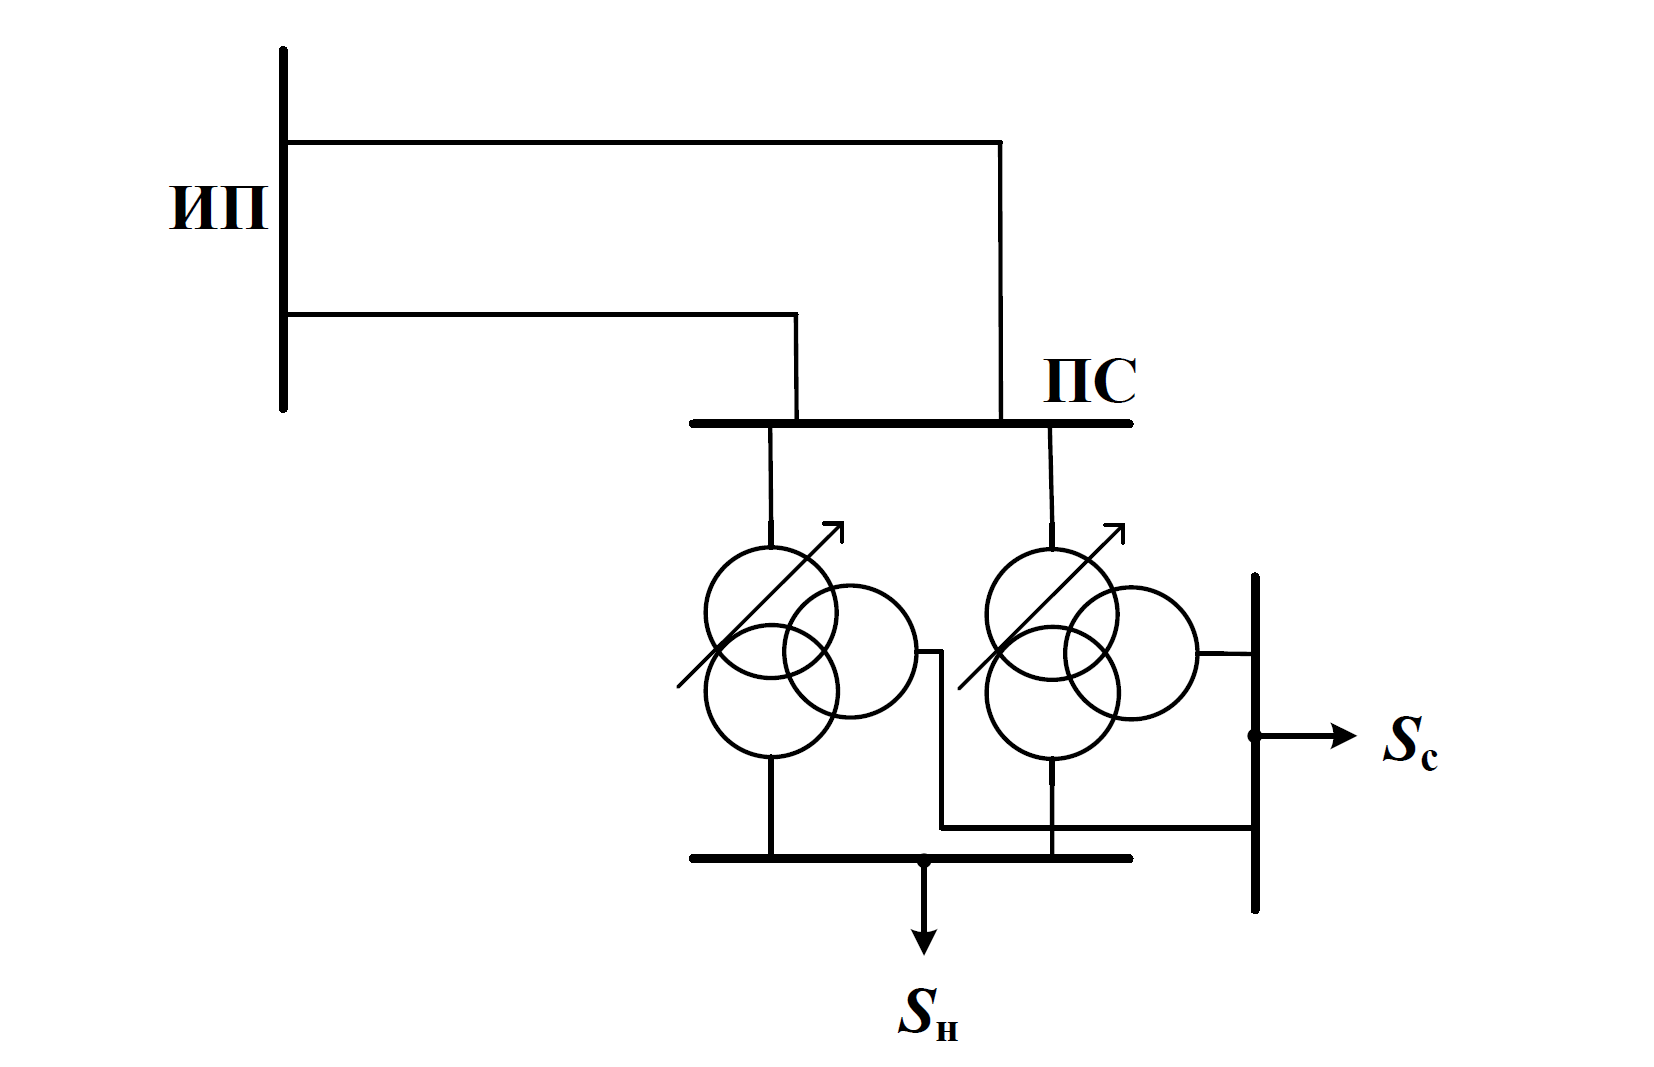
\includegraphics[width=0.9\textwidth]{inc/img/ish_dannie}
	\caption{Схема сети}
	\label{fig:scheme}
\end{figure}

Номинальное напряжение сети $U_{\text{ном}}$, марка проводов и длина линии $L_{\text{ИП-ПС}}$ от источника питания (ИП) до ПС, трансформаторы, установленные на ПС, приведены в табл.~\ref{tab:tabl1}. На шинах ИП района в режиме наибольших нагрузок обеспечивается напряжение, указанное в табл.~\ref{tab:tabl1} , а в режиме наименьших нагрузок 97 \% от номинального. Низшее напряжение на ПС составляет 10 кВ.

Мощность нагрузок на шинах низшего и среднего напряжений (НН и СН) ПС в режиме наибольших нагрузок ($P_{\text{н}}$ и $P_{\text{с}}$), наименьшая нагрузка (относительное снижение нагрузки $\alpha$) и число часов использования наибольших нагрузок $T_{\text{нб}}$ приведены в табл.~\ref{tab:tabl2}.

\renewcommand{\thetable}{\arabic{table}}
\begin{table}[H]
	\caption{Исходные данные для расчета (часть 1)}
	\begin{tabular}{|r|c|c|c|l|}
		\hline
		$U_{\text{ном}}$ , кВ & $U_{\text{ИП}}$, \% & $L_{\text{ИП-ПС}}$ & Марка провода & Трансформатор \\
		\hline
		110 & 113 & 84 & АС 150/24 & ТДТН-40000/110/35 \\
		\hline
	\end{tabular}
	\label{tab:tabl1}
\end{table}

\begin{table}[H]
	\caption{Исходные данные для расчета (часть 2)}
	\begin{tabular}{|r|c|c|c|c|l|}
		\hline
		$P_{c}$, кВт & $cos\varphi_c$ & $P_{\text{н}}$, кВт & $cos\varphi_{\text{н}} / tg\varphi_{\text{н}} $ & $\alpha$, отн. ед. & $T_{\text{нб}}$, ч/год \\
		\hline
		33000 & 0,82 & 22880 & - / 0,44 & 0,4 & 6820 \\
		\hline
	\end{tabular}
	\label{tab:tabl2}
\end{table}

По табл. 3.5 и 3.8 \cite{файбисович} определяем необходимые для расчета исходные данные по проводу АС 150/24 и сводим их в табл.~\ref{tab:tabl3}

\begin{table}[H]
	\caption{Расчетные данные сталеалюминевого провода АС 150/24}
	\begin{tabular}{|c|c|c|}
		\hline
		Номинальное сечение & Диаметр провода  & Активное сопротивление \\
		(алюминий/сталь) & $d_{\text{пр}}$, мм & постоянному току при \\
		провода, $\text{мм}^2$ & & температуре 20 $^{\circ}$C \\
		 & & $R_0$, Ом/км \\
		\hline
		150/24 & 17,1 & 0,204 \\
		\hline
	\end{tabular}
	\label{tab:tabl3}
\end{table}


\renewcommand{\thefigure}{\arabic{chapter}.\arabic{figure}} % возвращаем нормальную нумерацию картинок
\renewcommand{\thetable}{\arabic{chapter}.\arabic{table}} % возвращаем нормальную нумерацию таблиц

%%% Local Variables: 
%%% mode: latex
%%% TeX-master: "rpz"
%%% End: 

\mainmatter % это включает нумерацию глав и секций в документе ниже

\chapter{Составление схемы замещения сети и определение её параметров}
\label{cha:analysis}

Схема замещения изображенной на рис.~\ref{fig:scheme} электрической сети представляет взаимосвязанную совокупность схем замещения двухцепной воздушной линии (ВЛ) номинального напряжения 110 кВ и трехобмоточных трансформаторов ТДТН-40000/110/35. Сначала следует составить отдельные схемы замещения для каждого элемента электрической сети и рассчитать их параметры

\section{Схема замещения воздушной линии электропередачи}

Воздушные линии электропередачи напряжением 110 кВ допускается представлять П-образной схемой замещения, приведенной на рис.~\ref{fig:pobraz} \cite{веников1998электрические}. В этой схеме поперечные ветви с емкостной проводимостью заменены постоянными реактивными мощностями, равными половине зарядной мощности линии.

\begin{figure}
	\centering
	\includegraphics[width=0.7\textwidth]{inc/svg/zam_vl}
	\caption{П-образная схема замещения ВЛ 110 кВ}
	\label{fig:pobraz}
\end{figure}

Эквивалентное активное сопротивление линии рассчитывается по формуле:

\begin{eqndesc}[H]
	\begin{equation}
		R_\textup{л}=\frac{R_{\text{0}} \cdot L}{n_{\text{ц}}},
		\label{F:req}
	\end{equation}
	
	где $R_{\text{0}}$ "--- удельное активное сопротивление цепи, Ом/км, \\
		$L$ "--- длина линнии, км, \\
		$n_{\text{ц}}$ "--- количество цепей.
\end{eqndesc}

Рассчитаем по формуле \eqref{F:req} активное сопротивление линии ИП-ПС:

\[
R_{\text{ИП-ПС}} = \frac{R_{\text{0}} \cdot L_{\text{ИП-ПС}}}{n_{\text{ц ИП-ПС}}} = \frac{0,204\cdot84}{2} = 8,57\; \text{Ом}
\]

Эквивалентное индуктивное сопротивление линии определяется по формуле:

\begin{eqndesc}[H]
	\begin{equation}
		X_{\text{л}}=\frac{X_{\text{0}} \cdot L}{n_{\text{ц}}},
		\label{F:xeq}
	\end{equation}
	
	где $X_{\text{0}}$ "--- удельное индуктивное сопротивление цепи, Ом/км, определяемое в зависимости от
	среднегеометрического расстояния между проводами фаз линии $D_{\text{сг}}$ и радиуса провода
	$r_{\text{пр}} = \frac{d_{\text{пр}}}{2} = \frac{17,1}{2} = 8,55\; \text{мм}$.
\end{eqndesc}

\[
X_0 = 0,1445\, lg \frac{D_{\text{сг}}}{r_{\text{пр}}} + 0,0157 = 0,1445\, lg \frac{5000}{8,55} + 0,0157 = 0,416\; \frac{\text{Ом}}{\text{км}}
\]

Здесь принято значение усредненного среднегеометрического расстояния $D_{\text{сг}} = 5,0\; \text{м} = 5000\; \text{мм}$ согласно примечанию под таблицей 3.8 \cite{файбисович}.

Рассчитаем по формуле \eqref{F:xeq} индуктивное сопротивление линии ИП-ПС:
\[
X_{\text{ИП-ПС}} = \frac{X_{\text{0}} \cdot L_{\text{ИП-ПС}}}{n_{\text{ц ИП-ПС}}} = \frac{0,416\cdot84}{2} = 17,5\; \text{Ом}
\]

Эквивалентная емкостная проводимость линии:
\begin{eqndesc}[H]
	\begin{equation}
		B_{\text{л}} = n_{\text{ц}} \cdot B_0 \cdot L,
		\label{F:beq}
	\end{equation}

	где $B_0$ "--- удельная емкостная проводимость, См/км, которая так же, как и удельное индуктивное сопротивление, определяется в зависимости от среднегеометрического расстояния между проводами фаз линии $D_{\text{сг}}$ и радиуса провода $r_{\text{пр}}$. 

\end{eqndesc}

\[
B_0 = \frac{7,58\cdot 10^{-6}}{lg \frac{D_{\text{сг}}}{r_{\text{пр}}}} = \frac{7,58\cdot 10^{-6}}{lg \frac{5000}{8,55}} = 2,74\cdot 10^{-6}\; \frac{\text{См}}{\text{км}}
\]

Вычислим по формуле \eqref{F:beq} ёмкостную проводимость линии ИП-ПС:

\[
B_{\text{ИП-ПС}} = n_{\text{ц\, ИП-ПС}} \cdot B_0 \cdot L_{\text{ИП-ПС}} = 2 \cdot 2,74 \cdot 84 = 460,3\cdot 10^{-6}\; \text{См}
\]

Половина зарядной мощности линии 110 кВ:
\begin{eqndesc}[H]
	\begin{equation}
		\frac{Q_{\text{сл}}}{2} = \frac{n_{\text{ц}}\cdot Q_{c0}\cdot L}{2},
		\label{F:Q/2}
	\end{equation}
	где $Q_{c0}$ – удельная зарядная мощность линии, МВар/км.
\end{eqndesc}

Удельная зарядная мощность, соответствующая номинальному напряжению рассматриваемой ВЛ 110 кВ:
\[
Q_{c0} = U_{\text{ном}}^2 \cdot B_0 = 110^2 \cdot 2,74\cdot 10^{-6} = 0,0332\; \frac{\text{МВар}}{\text{км}}
\]

Рассчитаем по формуле \eqref{F:Q/2} половину эквивалентной зарядной мощности двухцепной линии ИП-ПС:
\[
\frac{Q_{c{\text{ИП-ПС}}}}{2} = \frac{n_{\text{ц\, ИП-ПС}}\cdot Q_{c0}\cdot L_{\text{ИП-ПС}}}{2} = \frac{2\cdot 0,0332\cdot 84}{2} = 2,78\; \text{МВар}
\]

Параметры схемы замещения воздушной линии электропередачи определены.

\section{Схема замещения трёхобмоточных трансформаторов}

Составим трехлучевую схему замещения двух параллельно работающих трансформаторов и определим её параметры (см рис. \ref{fig:t_obraz}).

Номинальная мощность трансформатора, номинальные напряжения обмоток, относительное напряжение короткого замыкания лучей, активные потери холостого хода трансформатора и относительное значение тока холостого хода приведены в табл. \ref{tab:tabl4}.

\newpage

\begin{figure}[h]
	\centering
	\includegraphics[width=0.7\textwidth]{inc/svg/t_obraz}
	\caption{Т-образная схема замещения двух параллельно работающих трансформаторов}
	\label{fig:t_obraz}
\end{figure}

\begin{table}[ht]
	\caption{Каталожные данные трансформатора ТДТН-40000/110/35}
	\begin{tabularx}{\textwidth}{|X|X|X|X|X|X|X|X|X|X|}
		\hline
		$S_{\text{т.ном}}$, МВА & \multicolumn{3}{c|}{$U_{\text{ном}}$, обмоток кВ} & \multicolumn{3}{c|}{$U_k$ \%} & $\Delta P_k$, кВт & $\Delta P_\textup{х}$, кВт   & $I_\textup{х}$, \%            \\ \hline
		\multirow{2}{*}{40}   & ВН  & СН   & НН                                   & ВН-СН & ВН-НН & СН-НН         & ВН-СН             & \multirow{2}{*}{43} & \multirow{2}{*}{0,6} \\ \cline{2-8}
		                      & 115 & 38,5 & 11                                   & 10,5  & 17    & 6             & 200               &                     &                      \\ \hline
	\end{tabularx}
	\label{tab:tabl4}
\end{table}

Рассчитаем эквивалентное активное сопротивление лучей высшего, среднего и низшего напряжений схемы замещения для двух трансформаторов:
\begin{eqndesc}[H]
	\begin{equation*}
		\begin{split}
			R_{\text{т.н.экв}} &= R_{\text{т.в.экв}} = R_{\text{т.с.экв}} = \frac{1}{n_{\text{т}}}\cdot \frac{\Delta P_{\text{к.в-с}}}{2}\cdot \frac{U_{\text{ВН}}^2}{S_{\text{т.ном}}^2} = \\
			& = \frac{1}{2}\cdot \frac{200\cdot 10^{-3}}{2}\cdot \frac{115^2}{40^2} = 0,413\; \text{Ом}
		\end{split}
	\end{equation*}

	где $\Delta P_{\text{к.в-с}}$ "--- потери активной мощности, соответствующие опыту короткого замыкания для обмоток высшего и среднего напряжений при разомкнутой обмотке низшего напряжения, МВт; \\
	$S_{\text{т.ном}}$ "--- номинальная мощность трансформатора, МВА; \\
	$U_{\text{ВН}}$ "--- номинальное напряжение обмотки высшего напряжения, кВ; \\
	$n_{\text{т}}$ "--- количество трансформаторов.
	
\end{eqndesc}

Рассчитаем относительные напряжения короткого замыкания обмоток высшего, среднего и низшего напряжений:
\begin{equation*} 
	U_{\text{к.в}} = 0,5\cdot \left(U_{\text{к\, в-с}} + U_{\text{к\, в-н}} - U_{\text{к\, c-н}}\right) =
	0,5 \cdot (10,5+17-6) = 10,8\; \%
\end{equation*}
\begin{equation*} 
	U_{\text{к.с}} = 0,5\cdot \left(U_{\text{к\, в-с}} + U_{\text{к\, с-н}} - U_{\text{к\, в-н}}\right) =
	0,5 \cdot (10,5+6-17) = 0\; \%
\end{equation*}
\begin{equation*} 
	U_{\text{к.н}} = 0,5\cdot \left(U_{\text{к\, с-н}} + U_{\text{к\, в-н}} - U_{\text{к\, в-с}}\right) =
	0,5 \cdot (6+17-10,5) = 6,25\; \%
\end{equation*}

Рассчитаем эквивалентное индуктивное сопротивление высшего, среднего и низшего напряжения лучевой схемы замещения для двух трансформаторов:
\begin{equation*}
	X_{\text{т.в.экв}} = \frac{1}{n_{\text{т}}}\cdot \frac{U_{\text{к.в}}}{100}\cdot \frac{U_{\text{ВН}}^2}{S_{\text{т.ном}}} = \frac{1}{2}\cdot \frac{10,8}{100}\cdot \frac{115^2}{40} = 17,9\; \text{Ом}
\end{equation*}
\begin{equation*}
	X_{\text{т.с.экв}} = \frac{1}{n_{\text{т}}}\cdot \frac{U_{\text{к.с}}}{100}\cdot \frac{U_{\text{ВН}}^2}{S_{\text{т.ном}}} = \frac{1}{2}\cdot \frac{0}{100}\cdot \frac{115^2}{40} = 0\; \text{Ом}
\end{equation*}
\begin{equation*}
	X_{\text{т.н.экв}} = \frac{1}{n_{\text{т}}}\cdot \frac{U_{\text{к.н}}}{100}\cdot \frac{U_{\text{ВН}}^2}{S_{\text{т.ном}}} = \frac{1}{2}\cdot \frac{6,25}{100}\cdot \frac{115^2}{40} = 10,3\; \text{Ом}
\end{equation*}

Рассчитаем эквивалентные потери активной мощности в двух трансформаторах при холостом ходе:
\begin{eqndesc}
	\begin{equation*}
		\Delta P_{\text{x.экв}} = n_{\text{т}}\cdot \Delta P_{\text{х}} = 2\cdot 43 = 86\; \text{кВт},
	\end{equation*}
	где $\Delta P_{\text{х}}$ "--- активные потери холостого хода, кВт.
\end{eqndesc}

Рассчитаем эквивалентные потери реактивной мощности в двух трансформаторах при холостом ходе по формуле:
\begin{eqndesc}
	\begin{equation*}
		\Delta Q_{\text{x.экв}} = n_{\text{т}}\cdot \frac{I_x}{100}\cdot S_{\text{т.ном}} = 2\cdot \frac{0,6}{100}\cdot 40 = 0,48\; \text{МВар}
	\end{equation*}
	где $I_{\text{х}}$ "--- относительное значения тока холостого хода, \%.
\end{eqndesc}

\section{Общая схема замещения сети}

Составим на рис. \ref{fig:obshaya_schema} общую схему замещения сети, состоящую из двух параллельно работающих трансформаторов и линии ВЛ 110 кВ, и укажем на ней все числовые значения рассчитанных параметров и их размерностей.

\begin{sidewaysfigure}
	\centering
	\includegraphics[width=0.9\textwidth]{inc/svg/obshaya_schema}
	\caption{Общая схема замещения двух параллельно работающих трансформаторов и ВЛ}
	\label{fig:obshaya_schema}
\end{sidewaysfigure}
%%% Local Variables:
%%% mode: latex
%%% TeX-master: "rpz"
%%% End:

\chapter{Расчет потокораспределения и напряжений в узлах сети в нормальном режиме наибольших нагрузок}
\label{cha:30-high_loads}

\section{Расчет нагрузок на шинах низшего и среднего напряжений подстанции}

Возьмем значения активной мощности на шинах низшего и среднего напряжений, $tg\varphi_\textup{н}$ и $cos\varphi_\textup{с}$ из табл. \ref*{tab:tabl2}.

Активная нагрузка на шинах низшего напряжения (НН): $P_\textup{н} = 22,9 \; \text{МВт}$

Реактивная нагрузка на шинах НН вычисляется по формуле:
\begin{eqndesc}
	\begin{equation*}
		Q_\textup{н} = P_\textup{н}\cdot tg\varphi_\textup{н} = 22,9\cdot 0,44 = 10,1\; \text{МВар},
	\end{equation*}

	где $P_\textup{н}$ "--- активная нагрузка на шинах НН; \\
	$tg_{\varphi_{\text{н}}}$ "--- коэффициент реактивной мощности.
\end{eqndesc}

Активная нагрузка на шинах среднего напряжения (СН): $P_\textup{с} = 33\; \text{МВт}$

Реактивная нагрузка на шинах СН:
\begin{eqndesc}
	\begin{equation*}
		Q_\textup{с} = \sqrt{S_c^2 - P_c^2} = \sqrt{\left(\frac{P_c}{cos\varphi_c}\right)^2 - P_c^2} = \sqrt{\left(\frac{33}{0,82}\right)^2 - 33^2} = 23,0\; \text{Мвар},
	\end{equation*}

	где $P_\textup{с}$ "--- активная мощность нагрузки на шинах СН; \\
	$cos_{\varphi_{\text{с}}}$ "--- коэффициент мощности нагрузки; \\
	$S_\textup{с}$ "--- полная мощность на шинах СН.
\end{eqndesc}


\section{Расчет режима наибольших нагрузок}

Найдем напряжение ИП-ПС:
\[U_\textup{ИП-ПС} = U_\textup{ном} \cdot U_\textup{ИП}, \% = 110\cdot 1,13 = 124,3\; \text{кВ}\]

\newpage
\textbf{1 этап}

В качестве начального приближения зададимся значениями напряжений на шинах СН и ВН, приведенными к стороне ВН, а так же напряжения в средней точке схемы замещения трансформатора (далее ТР), равными номинальному напряжению:
\[U_\textup{в}^{(0)} = U_\textup{н}^{{'}(0)} = U_\textup{с}^{{'}(0)} = U_0^{(0)} = U_\textup{ном} = 110\; \text{кВ}\]

\textbf{Луч среднего напряжения}

Мощность в конце луча СН:
\[S_c^{''} = P_c + jQ_c = 33,0 + j23,0 \; \text{МВА} \]

Потери мощности в сопротивлении по данным конца в общем виде рассчитываются по формуле:
\begin{eqndesc}[h]
	\begin{equation}
		\Delta S_{ij} = \left(\frac{S_{ij}^{''}}{U_{j}}\right)^2 \cdot Z_{ij}
		\label{eq:dS12}
	\end{equation}

	где $S_{ij}^{''}$ \--- мощность в конце участка \textit{i-j}, МВА, \\
	$U_j$ \--- напряжение в конце участка \textit{i-j}, кВ, \\
	$Z_{ij}$ \--- сопротивление участка \textit{i-j}, Ом.
\end{eqndesc}

Определим потери мощности в сопротивлении луча СН по формуле \eqref{eq:dS12}:
\[\Delta S_c = \frac{(S_c^{''})^2}{U_\textup{ном}^2}\cdot Z_c = \frac{33^2+23^2}{110^2}\cdot 0,413 = 0,055\; \text{МВт}\]

Определим мощность в начале луча СН:
\[S_c^{'} = S_c^{''} + \Delta S_c = 33,0 + j23,0 + 0,055 = 33,1 + j23,0\; \text{МВА}\]

\textbf{Луч низшего напряжения}

Мощность в конце луча НН:
\[S_\textup{н}^{''} = P_\textup{н} + jQ_\textup{н} = 22,9 + j10,1 \; \text{МВА}\]

Потери мощности в сопротивлении луча НН:
\[\Delta S_\textup{н} = \frac{(S_\textup{н}^{''})^2}{U_\textup{ном}^2}\cdot Z_\textup{н} = \frac{22,9^2+10,1^2}{110^2}\cdot (0,413 + j10,3) = 0,0214 + j0,533\; \text{МВА}\]

Определим мощность в начале луча НН:
\[S_\textup{н}^{'} = S_\textup{н}^{''} + \Delta S_\textup{н} = 22,9 + j10,1 + 0,0214 + j0,533 = 22,9 + j10,6 \; \text{МВА}\]

\textbf{Луч высшего напряжения}

Мощность в конце луча ВН:
\[S_\textup{в}^{''} = S_c^{'} + S_\textup{в}^{'} = 33,1 + j23,0 + 22,9 + j10,6 = 56,0 + j33,6 \; \text{МВА}\]

Потери мощности в сопротивлении луча ВН:
\[\Delta S_\textup{в} = \frac{(S_\textup{в}^{''})^2}{(U_\textup{ном})^2} \cdot Z_\textup{в} = \frac{56^2 + 33,6^2}{110^2} \cdot (0,413 + j17,9) = 0,146 + j6,31 \; \text{МВА} \]

Мощность в начале луча ВН:
\[S_\textup{в}^{'} = S_\textup{в}^{''} + \Delta S_\textup{в} = 56,0 + j33,6 + 0,146 + j6,31 = 56,1 + j39,9\; \text{МВА}\]

Приведенная нагрузка подстанции:
\[S_\textup{прив} = S_\textup{в}^{'} + \Delta S_\textup{х} = 56,1 + j39,9 + 0,086 + j0,48 = 56,2 + j40,4 \; \text{МВА}\]

Зарядная мощность в конце линии ИП-ПС:
\[\frac{Q_\textup{с.ИП-ПС}^{''}}{2} = \frac{U_\textup{ном}^2\cdot B_\textup{л}}{2} = \frac{110^2 \cdot 460,3\cdot 10^{-6}}{2} = 2,78\; \text{МВар} \]

Расчетная нагрузка подстанции:
\[S_p = S_\textup{прив} - j\frac{Q_\textup{с.ИП-ПС}^{''}}{2} = 56,2 + j40,4 - j2,78 = 56,2 + j37,6\; \text{МВА}\]

Мощность в конце линии ИП-ПС:
\[S_\textup{ИП-ПС}^{''} = S_p = 56,2 + j37,6\; \text{МВА}\]

Потери мощности в сопротивлении линии ИП:
\[\Delta S_\textup{ИП-ПС} = \frac{\left(S_\textup{ИП-ПС}^{''}\right)^2}{U_\textup{ном}^2}\cdot Z_\textup{л} = \frac{56,2^2 + 37,6^2}{110^2} \cdot (8,57 + j17,5) = 3,24 + j6,61 \; \text{МВА}\]

Мощность в начале линии ИП-ПС:
\[S_\textup{ИП-ПС}^{'} = S_\textup{ИП-ПС}^{''} + \Delta S_\textup{ИП-ПС} = 56,2 + j37,6 + 3,24 + j6,61 = 59,4 + j44,2 \; \text{МВА}\]

Зарядная мощность в начале линии ИП-ПС:
\[\frac{Q_\textup{с.ИП-ПС}^{'}}{2} = \frac{U_\textup{ИП-ПС}^2\cdot B_\textup{л}}{2} = \frac{124,3^2 \cdot 460,3\cdot 10^{-6}}{2} = 3,56\; \text{МВар}\]

Мощность, выдаваемая источником в сеть:
\[S_\textup{ИП-ПС} = S_\textup{ИП-ПС}^{'} - j\frac{Q_\textup{с.ИП-ПС}^{'}}{2} = 59,4 + j44,2 - j3,56 = 59,4 + 40,6\; \text{МВА}\]

\textbf{2 этап}

Продольная составляющая вектора падения напряжения по данным начала находится по формуле:

\begin{equation}
	\Delta U_{ij} = \frac{P_{ij}^{'}\cdot R_{ij} + Q_{ij}^{'}\cdot X_{ij}}{U_{i}}
\end{equation}

Поперечной составляющей можем пренебречь, так как линия класса напряжения 110 кВ.

Продольная составляющая вектора падения напряжения на сопротивлении линии ИП-ПС:
\[\Delta U_\textup{ИП-ПС} = \frac{P_\textup{ИП-ПС}^{'}\cdot R_\textup{л} + Q_\textup{ИП-ПС}^{'}\cdot X_\textup{л}}{U_\textup{ИП-ПС}} = \frac{59,4\cdot 8,57 + 44,2\cdot 17,5}{124,3} = 10,3\; \text{кВ}\]

Напряжение на шинах ВН:
\[U_\textup{в} = U_\textup{ИП-ПС} - \Delta U_\textup{ИП-ПС} = 124,3 - 10,3 = 114,0 \; \text{кВ}\]

Продольная составляющая вектора падения напряжения на сопротивлении луча высшего напряжения:
\[\Delta U_\textup{в} = \frac{P_\textup{в}^{'}\cdot R_\textup{т.в} + Q_\textup{в}^{'}\cdot X_\textup{т.в}}{U_\textup{в}} = \frac{56,1\cdot 0,413 + 39,9\cdot 17,9}{114,0} = 6,47\; \text{кВ}\]

Напряжение в средней точке cхемы замещения трансформаторов:
\[U_\textup{0} = U_\textup{в} - \Delta U_\textup{в} = 114,0 - 6,47 = 107,5 \; \text{кВ}\]

Продольная составляющая вектора падения напряжения на сопротивлении луча среднего напряжения:
\[\Delta U_\textup{с} = \frac{P_\textup{с}^{'}\cdot R_\textup{т.с} + Q_\textup{с}^{'}\cdot X_\textup{т.с}}{U_\textup{0}} = \frac{33,1\cdot 0,413 + 23,0\cdot 0}{107,5} = 0,127\; \text{кВ}\]

Напряжение на шинах СН, приведенное к стороне ВН:
\[U_\textup{с}^{'} = U_\textup{0} - \Delta U_\textup{н} = 107,5 - 0,127 = 107,4 \; \text{кВ}\]

Продольная составляющая вектора падения напряжения на сопротивлении луча низшего напряжения:
\[\Delta U_\textup{н} = \frac{P_\textup{н}^{'}\cdot R_\textup{т.н} + Q_\textup{н}^{'}\cdot X_\textup{т.н}}{U_\textup{0}} = \frac{22,9\cdot 0,413 + 10,6\cdot 10,3}{107,5} = 1,10\; \text{кВ}\]

Напряжение на шинах НН, приведенное к стороне ВН:
\[U_\textup{н}^{'} = U_\textup{0} - \Delta U_\textup{н} = 107,5 - 1,10 = 106,4 \; \text{кВ}\]

Полная расчетная схема замещения сети в нормальном режиме наибольшей нагрузки изображена на рис. \ref{fig:rezhim_NB}. 

\begin{sidewaysfigure}
	\centering
	\includegraphics[width=0.9\textwidth]{inc/svg/rezhim_NB}
	\caption{Полная схема замещения сети для режима наибольших нагрузок}
	\label{fig:rezhim_NB}
\end{sidewaysfigure}
%%% Local Variables:
%%% mode: latex
%%% TeX-master: "rpz"
%%% End:
\chapter{Расчет потокораспределения и напряжений в узлах сети в нормальном режиме наименьших нагрузок}
\label{cha:40-low_loads}

\section{Расчет нагрузок на шинах низшего и среднего напряжений подстанции}

Возьмем значения активной мощности на шинах низшего и среднего напряжений, $tg\varphi_\textup{н}$ и $cos\varphi_\textup{с}$ из табл. \ref*{tab:tabl2}.

Активная нагрузка на шинах низшего напряжения (НН): $P_\textup{н} = 22,9 \cdot \alpha = 22,9\cdot 0,4 = 9,16 \; \text{МВт}$

Реактивная нагрузка на шинах НН вычисляется по формуле:
\begin{eqndesc}
	\begin{equation*}
		Q_\textup{н} = P_\textup{н}\cdot tg\varphi_\textup{н}\cdot \alpha = 22,9\cdot 0,44\cdot 0,4 = 4,03\; \text{МВар},
	\end{equation*}
	
	где $P_\textup{н}$ "--- активная нагрузка на шинах НН, \\
	$tg_{\varphi_{\text{н}}}$ "--- коэффициент реактивной мощности.
\end{eqndesc}

Активная нагрузка на шинах среднего напряжения (СН): $P_\textup{с} = 33\cdot 0,4 = 13,2\; \text{МВт}$

Реактивная нагрузка на шинах НН вычисляется по формуле:
\begin{eqndesc}
	\begin{equation*}
		Q_\textup{с} = \sqrt{S_c^2 - P_c^2} = \sqrt{\left(\frac{P_c}{cos\varphi_c}\right)^2 - P_c^2} = \sqrt{\left(\frac{13,2}{0,82}\right)^2 - 13,2^2} = 9,21\; \text{Мвар},
	\end{equation*}
	
	где $P_\textup{с}$ "--- активная мощность нагрузки на шинах СН, \\
	$cos_{\varphi_{\text{с}}}$ "--- коэффициент мощности нагрузки, \\
	$S_\textup{с}$ "--- полная мощность на шинах СН.
\end{eqndesc}

\section{Расчет режима наименьших нагрузок}

По условию, напряжение на источнике питания в режиме наименьших нагрузок составляет 97\%. Найдем напряжение ИП-ПС:
\[U_\textup{ИП-ПС} = U_\textup{ном} \cdot U_\textup{ИП}, \% = 110\cdot 0,97 = 106,7\; \text{кВ}\]

\textbf{1 этап}

В качестве начального приближения зададимся значениями напряжений на шинах СН и ВН, приведенными к стороне ВН, а так же напряжения в средней точке схемы замещения ТР, равными номинальному напряжению:
\[U_\textup{в}^{(0)} = U_\textup{н}^{{'}(0)} = U_\textup{с}^{{'}(0)} = U_0^{(0)} = U_\textup{ном} = 110\; \text{кВ}\]

\textbf{Луч среднего напряжения}

Мощность в конце луча СН:
\[S_c^{''} = P_c + jQ_c = 13,2 + j9,21 \; \text{МВА} \]

%Потеря мощности в сопротивлении рассчитывается по формуле:
%\begin{eqndesc}
%	\begin{equation}
%		\Delta S_{12} = \left(\frac{S_{12}^{(')('')}}{U_{(1)(2)}}\right)^2 \cdot Z_{12}
%		\label{eq:dS12}
%	\end{equation}
%	
%	где $S_12^{'}$ \--- мощность в начале участка 1-2, МВА, \\
%	$S_12^{''}$ \--- мощность в конце участка 1-2, МВА, \\
%	$U_1$ \--- напряжение в начале участка 1-2, кВ, \\
%	$U_2$ \--- напряжение в конце участка 1-2, кВ, \\
%	$Z_{12}$ \--- сопротивление участка 1-2, Ом.
%\end{eqndesc}

Определим потери мощности в сопротивлении луча СН по формуле \eqref{eq:dS12}:
\[\Delta S_c = \frac{(S_c^{''})^2}{U_\textup{ном}^2}\cdot Z_c = \frac{13,2^2+9,21^2}{110^2}\cdot 0,413 = 0,00884\; \text{МВт}\]

Определим мощность в начале луча СН:
\[S_c^{'} = S_c^{''} + \Delta S_c = 13,2 + j9,21 + 0,00884 = 13,2 + j9,21\; \text{МВА}\]

\textbf{Луч низшего напряжения}

Мощность в конце луча НН:
\[S_\textup{н}^{''} = P_\textup{н} + jQ_\textup{н} = 9,16 + j4,03 \; \text{МВА}\]

Потери мощности в сопротивлении луча НН:
\[\Delta S_\textup{н} = \frac{(S_\textup{н}^{''})^2}{U_\textup{ном}^2}\cdot Z_\textup{н} = \frac{9,16^2+4,03^2}{110^2}\cdot (0,413 + j10,3) = 0,00342 + j0,0853\; \text{МВА}\]

Определим мощность в начале луча НН:
\[S_\textup{н}^{'} = S_\textup{н}^{''} + \Delta S_\textup{н} = 9,16 + j4,03 + 0,00342 + j0,0853 = 9,16 + j4,12\; \text{МВА}\]

\newpage
\textbf{Луч высшего напряжения}

Мощность в конце луча ВН:
\[S_\textup{в}^{''} = S_c^{'} + S_\textup{в}^{'} = 13,2 + j9,21 + 9,16 + j4,12 = 22,4 + j13,3\; \text{МВА}\]

Потери мощности в сопротивлении луча ВН:
\[\Delta S_\textup{в} = \frac{(S_\textup{в}^{''})^2}{(U_\textup{ном})^2} \cdot Z_\textup{в} = \frac{22,4^2 + 13,3^2}{110^2} \cdot (0,413 + j17,9) = 0,0232 + j1,00\; \text{МВА} \]

Мощность в начале луча ВН:
\[S_\textup{в}^{'} = S_\textup{в}^{''} + \Delta S_\textup{в} = 22,4 + j13,3 + 0,0232 + j1,00 = 22,4 + j14,3\; \text{МВА}\]

Приведенная нагрузка подстанции:
\[S_\textup{прив} = S_\textup{в}^{'} + \Delta S_\textup{х} = 22,4 + j14,3 + 0,086 + j0,48 = 22,5 + j14,8\; \text{МВА}\]

Зарядная мощность в конце линии ИП-ПС:
\[\frac{Q_\textup{с.ИП-ПС}^{''}}{2} = \frac{U_\textup{ном}^2\cdot B_\textup{л}}{2} = \frac{110^2 \cdot 460,3\cdot 10^{-6}}{2} = 2,78\; \text{МВар} \]

Расчетная нагрузка подстанции:
\[S_p = S_\textup{прив} - j\frac{Q_\textup{с.ИП-ПС}^{''}}{2} = 22,5 + j14,8 - j2,78 = 22,5 + j12,0\; \text{МВА}\]

Мощность в конце линии ИП-ПС:
\[S_\textup{ИП-ПС}^{''} = S_p = 22,5 + j12,0\; \text{МВА}\]

Потери мощности в сопротивлении линии ИП:
\[\Delta S_\textup{ИП-ПС} = \frac{\left(S_\textup{ИП-ПС}^{''}\right)^2}{U_\textup{ном}^2}\cdot Z_\textup{л} = \frac{22,5^2 + 12,0^2}{110^2} \cdot (8,57 + j17,5) = 0,461 + j0,940\; \text{МВА}\]

Мощность в начале линии ИП-ПС:
\[S_\textup{ИП-ПС}^{'} = S_\textup{ИП-ПС}^{''} + \Delta S_\textup{ИП-ПС} = 22,5 + j12,0 + 0,461 + j0,940 = 23,0 + j12,9\; \text{МВА}\]

Зарядная мощность в начале линии ИП-ПС:
\[\frac{Q_\textup{с.ИП-ПС}^{'}}{2} = \frac{U_\textup{ИП-ПС}^2\cdot B_\textup{л}}{2} = \frac{106,7^2 \cdot 460,3\cdot 10^{-6}}{2} = 2,62\; \text{МВар}\]

Мощность, выдаваемая источником в сеть:
\[S_\textup{ИП-ПС} = S_\textup{ИП-ПС}^{'} - j\frac{Q_\textup{с.ИП-ПС}^{'}}{2} = 23,0 + j12,9 - j2,62 = 23,0 + j10,3\; \text{МВА}\]

\textbf{2 этап}

%Продольная составляющая вектора падения напряжения находится по формуле:
%
%\begin{equation}
%	\Delta U_{12} = \frac{P_{12}^{(')('')}\cdot R_{12} + Q_{12}^{(')('')}\cdot X_{12}}{U_{(1)(2)}}
%\end{equation}
%
Поперечной составляющей можем пренебречь, так как линия класса напряжения 110 кВ.

Продольная составляющая вектора падения напряжения на сопротивлении линии ИП-ПС:
\[\Delta U_\textup{ИП-ПС} = \frac{P_\textup{ИП-ПС}^{'}\cdot R_\textup{л} + Q_\textup{ИП-ПС}^{'}\cdot X_\textup{л}}{U_\textup{ИП-ПС}} = \frac{23,0\cdot 8,57 + 12,9\cdot 17,5}{106,7} = 3,96\; \text{кВ}\]

Напряжение на шинах ВН:
\[U_\textup{в} = U_\textup{ИП-ПС} - \Delta U_\textup{ИП-ПС} = 106,7 - 3,96 =  102,7\; \text{кВ}\]

Продольная составляющая вектора падения напряжения на сопротивлении луча высшего напряжения:
\[\Delta U_\textup{в} = \frac{P_\textup{в}^{'}\cdot R_\textup{т.в} + Q_\textup{в}^{'}\cdot X_\textup{т.в}}{U_\textup{в}} = \frac{22,4\cdot 0,413 + 14,3\cdot 17,9}{102,7} = 2,58\; \text{кВ}\]

Напряжение в средней точке схемы замещения трансформаторов:
\[U_\textup{0} = U_\textup{в} - \Delta U_\textup{в} = 102,7 - 2,58 = 100,1\; \text{кВ}\]

Продольная составляющая вектора падения напряжения на сопротивлении луча среднего напряжения:
\[\Delta U_\textup{с} = \frac{P_\textup{с}^{'}\cdot R_\textup{т.с} + Q_\textup{с}^{'}\cdot X_\textup{т.с}}{U_\textup{0}} = \frac{13,2\cdot 0,413 + 9,21\cdot 0}{100,1} = 0,0545\; \text{кВ}\]

Напряжение на шинах СН, приведенное к стороне ВН:
\[U_\textup{с}^{'} = U_\textup{0} - \Delta U_\textup{н} = 100,1 - 0,0545 = 100,0 \; \text{кВ}\]

Продольная составляющая вектора падения напряжения на сопротивлении луча низшего напряжения:
\[\Delta U_\textup{н} = \frac{P_\textup{н}^{'}\cdot R_\textup{т.н} + Q_\textup{н}^{'}\cdot X_\textup{т.н}}{U_\textup{0}} = \frac{9,16\cdot 0,413 + 4,12\cdot 10,3}{100,1} = 0,462\; \text{кВ}\]

Напряжение на шинах НН, приведенное к стороне ВН:
\[U_\textup{н}^{'} = U_\textup{0} - \Delta U_\textup{н} = 100,1 - 0,462 = 99,6 \; \text{кВ}\]

Полная расчетная схема замещения сети в нормальном режиме наименьшей нагрузки приведена на рис. \ref{fig:rezhim_NM}. 

\begin{sidewaysfigure}
	\centering
	\includegraphics[width=0.9\textwidth]{inc/svg/rezhim_NM}
	\caption{Полная схема замещения сети в режиме наименьших нагрузок}
	\label{fig:rezhim_NM}
\end{sidewaysfigure}
\chapter{Расчет потокораспределения и напряжений в узлах сети в послеаварийном режиме}
\label{cha:50-emergency}

Поскольку в послеаварийном режиме одна цепь линии ИП-ПС отключена, пересчитаем активное и индуктивное сопротивления линии ИП-ПС:
\[R_\textup{ИП-ПС} = \frac{R_0\cdot L_\textup{ИП-ПС}}{n_\textup{ц\, ИП-ПС}} = \frac{0,204\cdot 84}{1} = 17,1\; \text{Ом}\]
\[X_\textup{ИП-ПС} = \frac{X_0\cdot L_\textup{ИП-ПС}}{n_\textup{ц\, ИП-ПС}} = \frac{0,416\cdot 84}{1} = 34,9\; \text{Ом}\]

\section{Расчет нагрузок на шинах низшего и среднего напряжений подстанции}

Возьмем значения активной мощности на шинах низшего и среднего напряжений, $tg\varphi_\textup{н}$ и $cos\varphi_\textup{с}$ из табл. \ref*{tab:tabl2}.

Активная нагрузка на шинах низшего напряжения: $P_\textup{н} = 22,9 \; \text{МВт}$

Реактивная нагрузка на шинах НН вычисляется по формуле:
\begin{eqndesc}
	\begin{equation*}
		Q_\textup{н} = P_\textup{н}\cdot tg\varphi_\textup{н} = 22,9\cdot 0,44 = 10,1\; \text{МВар},
	\end{equation*}
	
	где $P_\textup{н}$ "--- активная нагрузка на шинах НН, \\
	$tg_{\varphi_{\text{н}}}$ "--- коэффициент реактивной мощности.
\end{eqndesc}

Активная нагрузка на шинах среднего напряжения (СН): $P_\textup{с} = 33\; \text{МВт}$

Реактивная нагрузка на шинах СН:
\begin{eqndesc}
	\begin{equation*}
		Q_\textup{с} = \sqrt{S_c^2 - P_c^2} = \sqrt{\left(\frac{P_c}{cos\varphi_c}\right)^2 - P_c^2} = \sqrt{\left(\frac{33}{0,82}\right)^2 - 33^2} = 23,0\; \text{Мвар},
	\end{equation*}
	
	где $P_\textup{с}$ "--- активная мощность нагрузки на шинах СН, \\
	$cos_{\varphi_{\text{с}}}$ "--- коэффициент мощности нагрузки, \\
	$S_\textup{с}$ "--- полная мощность на шинах СН.
\end{eqndesc}

\section{Расчет послеаварийного режима}
\textbf{1 этап}

Расчет первого этапа до определения зарядной мощности идентичен разделу \ref{cha:30-high_loads}.

Зарядная мощность в конце линии ИП-ПС уменьшиться в два раза, т.к. $n_\textup{ц}=1$:
\[\frac{Q_\textup{с.ИП-ПС}^{''}}{2} = \frac{1}{2}\cdot \frac{U_\textup{ном}^2\cdot B_\textup{л}}{2} = \frac{1}{2}\cdot \frac{110^2 \cdot 460,3\cdot 10^{-6}}{2} = 1,39\; \text{МВар} \]

Расчетная нагрузка подстанции:
\[S_p = S_\textup{прив} - j\frac{Q_\textup{с.ИП-ПС}^{''}}{2} = 56,2 + j40,4 - j1,39 = 56,2 + j39,0\; \text{МВА}\]

Мощность в конце линии ИП-ПС:
\[S_\textup{ИП-ПС}^{''} = S_p = 56,2 + j39,0\; \text{МВА}\]

Потери мощности в сопротивлении линии ИП:
\[\Delta S_\textup{ИП-ПС} = \frac{\left(S_\textup{ИП-ПС}^{''}\right)^2}{U_\textup{ном}^2}\cdot Z_\textup{л} = \frac{56,2^2 + 39,0^2}{110^2} \cdot (17,1 + j34,9) = 6,61 + j13,5 \; \text{МВА}\]

Мощность в начале линии ИП-ПС:
\[S_\textup{ИП-ПС}^{'} = S_\textup{ИП-ПС}^{''} + \Delta S_\textup{ИП-ПС} = 56,2 + j39,0 + 6,61 + j13,5 = 62,8 + j52,5\; \text{МВА}\]

Зарядная мощность в начале линии ИП-ПС уменьшится в два раза, т.к. $n_\textup{ц}=1$:
\[\frac{Q_\textup{с.ИП-ПС}^{'}}{2} = \frac{1}{2}\cdot \frac{U_\textup{ИП-ПС}^2\cdot B_\textup{л}}{2} = \frac{1}{2}\cdot \frac{124,3^2 \cdot 460,3\cdot 10^{-6}}{2} = 1,78\; \text{МВар}\]

Мощность, выдаваемая источником в сеть:
\[S_\textup{ИП-ПС} = S_\textup{ИП-ПС}^{'} - j\frac{Q_\textup{с.ИП-ПС}^{'}}{2} = 62,8 + j52,5 - j1,78 = 62,8 + j50,7\; \text{МВА}\]

\newpage

\textbf{2 этап}

%Продольная составляющая вектора падения напряжения находится по формуле:
%
%\begin{equation}
%	\Delta U_{12} = \frac{P_{12}^{(')('')}\cdot R_{12} + Q_{12}^{(')('')}\cdot X_{12}}{U_{(1)(2)}}
%\end{equation}
%
%Поперечной составляющей можем пренебречь, так как у нас линия уровня напряжения 110 кВ.
%
Продольная составляющая вектора падения напряжения на сопротивлении линии ИП-ПС:
\[\Delta U_\textup{ИП-ПС} = \frac{P_\textup{ИП-ПС}^{'}\cdot R_\textup{л} + Q_\textup{ИП-ПС}^{'}\cdot X_\textup{л}}{U_\textup{ИП-ПС}} = \frac{62,8\cdot 17,1 + 52,5\cdot 34,9}{124,3} = 23,4\; \text{кВ}\]

Напряжение на шинах ВН:
\[U_\textup{в} = U_\textup{ИП-ПС} - \Delta U_\textup{ИП-ПС} = 124,3 - 23,4 = 100,9 \; \text{кВ}\]

Продольная составляющая вектора падения напряжения на сопротивлении луча высшего напряжения:
\[\Delta U_\textup{в} = \frac{P_\textup{в}^{'}\cdot R_\textup{т.в} + Q_\textup{в}^{'}\cdot X_\textup{т.в}}{U_\textup{в}} = \frac{56,1\cdot 0,413 + 39,9\cdot 17,9}{100,9} = 7,31\; \text{кВ}\]

Напряжение в средней точке схемы замещения трансформаторов:
\[U_\textup{0} = U_\textup{в} - \Delta U_\textup{в} = 100,9 - 7,31 = 93,6 \; \text{кВ}\]

Продольная составляющая вектора падения напряжения на сопротивлении луча среднего напряжения:
\[\Delta U_\textup{с} = \frac{P_\textup{с}^{'}\cdot R_\textup{т.с} + Q_\textup{с}^{'}\cdot X_\textup{т.с}}{U_\textup{0}} = \frac{33,1\cdot 0,413 + 23,0\cdot 0}{93,6} = 0,146\; \text{кВ}\]

Напряжение на шинах СН, приведенное к стороне ВН:
\[U_\textup{с}^{'} = U_\textup{0} - \Delta U_\textup{н} = 93,6 - 0,146 = 93,5 \; \text{кВ}\]

Продольная составляющая вектора падения напряжения на сопротивлении луча низшего напряжения:
\[\Delta U_\textup{н} = \frac{P_\textup{н}^{'}\cdot R_\textup{т.н} + Q_\textup{н}^{'}\cdot X_\textup{т.н}}{U_\textup{0}} = \frac{22,9\cdot 0,413 + 10,6\cdot 10,3}{93,6} = 1,27\; \text{кВ}\]

Напряжение на шинах НН, приведенное к стороне ВН:
\[U_\textup{н} = U_\textup{0} - \Delta U_\textup{н} = 93,6 - 1,27 = 92,3 \; \text{кВ}\]

Полная расчетная схема замещения сети в послеаварийном режиме показана на рис. \ref{fig:rezhim_emergency}

\begin{sidewaysfigure}
	\centering
	\includegraphics[width=0.9\textwidth]{inc/svg/rezhim_emergency}
	\caption{Полная схема замещения сети в послеаварийном режиме}
	\label{fig:rezhim_emergency}
\end{sidewaysfigure}

\chapter{Оценка достаточности регулировочных диапазонов устройств РПН трансформаторов на подстанции}
\label{cha:60-rpn}

Из расчёта режимов наименьших и наибольших нагрузок, а так же послеаварийного режима, известны значения напряжений на шинах среднего и низшего напряжений, приведённых к стороне высшего.

Режим наибольших нагрузок:
\[U_\textup{н.нб}^{'} = 106,4\; \text{кВ}; \qquad U_\textup{с.нб}^{'} = 107,4\; \text{кВ}\]

Режим наименьших нагрузок:
\[U_\textup{н.нм}^{'} = 99,6\; \text{кВ}; \qquad U_\textup{с.нм}^{'} = 100,0\; \text{кВ}\]

Послеаварийный режим:
\[U_\textup{н.п.ав}^{'} = 92,3\; \text{кВ}; \qquad U_\textup{с.п.ав}^{'} = 93,5\; \text{кВ}\]

Номинальные напряжения обмоток ВН, СН, НН трансформатора находим по табл. \ref{tab:tabl4}:
\[U_\textup{ВН.ном} = 115\; \text{кВ}; \qquad U_\textup{СН.ном} = 38,5\; \text{кВ}; \qquad U_\textup{НН.ном} = 11\; \text{кВ}\]

Диапазон регулирования РПН на стороне ВН: $\pm 9 \times 1,78 \%$

Диапазон регулирования ПБВ на стороне СН: $\pm 2 \times 2,5 \%$

Определим желаемый уровень напряжения на шинах СН $ 35\; \text{кВ}$.

Желаемое напряжение в режиме наибольших нагрузок:
\[U_\textup{с.нб}^\textup{жел} = 1,1 \cdot U_\textup{с.ном} = 1,1 \cdot 35 = 38,5\; \text{кВ}\]

Желаемое напряжение в режиме наименьших нагрузок:
\[U_\textup{с.нм}^\textup{жел} = 1,05 \cdot U_\textup{с.ном} = 1,05 \cdot 35 = 36,8\; \text{кВ}\]

В соответствии с п.1.2.23 ПУЭ \cite{пуэ7} устройства регулирования напряжения должны обеспечивать поддержание напряжения на шинах напряжением 3-20 кВ электростанций и подстанций, к которым присоединены распределительные сети, в пределах не ниже 105 \% номинального в период наибольших нагрузок и не выше 100 \% номинального в период наименьших нагрузок этих сетей.

Определим желаемый уровень напряжения на шинах НН $ 10\; \text{кВ}$.

Желаемое напряжение в режиме наибольших нагрузок:
\[U_\textup{н.нб}^\textup{жел} \geq 1,05 \cdot U_\textup{н.ном} = 1,05 \cdot 10 = 10,5\; \text{кВ}\]

Желаемое напряжение в режиме наименьших нагрузок:
\[U_\textup{н.нм}^\textup{жел} \leq 1,0 \cdot U_\textup{н.ном} = 1,0 \cdot 10 = 10,0\; \text{кВ}\]

\section{Режим наибольших нагрузок}

\textbf{Сторона НН}
 
Желаемое напряжение на шинах НН вычисляется по формуле:
\begin{eqndesc}
	\begin{equation}
		U_\textup{н}^\textup{жел} = \frac{U_\text{н}^{'}\cdot U_\textup{НН.ном}}{U_\text{ВН.ном}\cdot \left(1 + n_\textup{отв}^\textup{жел} \cdot \frac{\Delta U_\textup{отв}}{100\%}\right)},
		\label{F:U_zhelNN}
	\end{equation}

где $n_\textup{отв}^\textup{жел}$ "--- желаемое ответвление регулируемой части обмотки ВН; \\
$\Delta U_\textup{отв}$ "--- ступень регулирования одного ответвления в процентах.
\end{eqndesc}

Выразим из формулы \eqref{F:U_zhelNN} ответвление регулируемой части обмотки ВН, обеспечивающее желаемое напряжение на шинах НН в режиме наибольших нагрузок:
\[n_\textup{отв}^\textup{жел} \leq \left(\frac{U_\textup{н.нб}^{'}\cdot U_\textup{НН.ном}}{U_\textup{н.нб}^\textup{жел}\cdot U_\textup{ВН.ном} - 1}\right) \cdot \frac{100\%}{\Delta U_\textup{отв}} = \left(\frac{106,4\cdot 11}{10,5\cdot 115} - 1 \right) \cdot \frac{100\%}{1,78\%} = -1,73\]

Полученное значение округляем до целого числа с учетом знака неравенства и предельного количества ответвлений $(-9 \leq n_\textup{отв}^\textup{действ} \leq +9)$, то есть $n_\textup{отв}^\textup{действ} = -2$.

Рассчитаем действительное напряжение на шинах НН в режиме наибольших нагрузок:
\[U_\textup{н.нб}^\textup{действ} = \frac{U_\textup{н.нб}^{'}\cdot U_\textup{НН.ном}}{U_\textup{ВН.ном}\cdot \left(1 + n_\textup{отв}^\textup{действ} \cdot \frac{\Delta U_\textup{отв}}{100\%}\right)} = \frac{106,4\cdot 11}{115 \cdot \left(1 - 2 \cdot \frac{1,78\%}{100\%}\right)} = 10,55\; \text{кВ}\]

\textbf{Сторона СН}

Желаемое напряжение на шинах СН находится по формуле:
\begin{eqndesc}
	\begin{equation}
		U_\textup{с}^\textup{жел} = \frac{U_\textup{с}^{'}\cdot U_\textup{СН.ном}}{U_\textup{ВН.ном}\cdot \left(1 + n_\textup{отв}^\textup{действ} \cdot \frac{\Delta U_\textup{отв}}{100\%}\right)} \cdot \left(1 + n_\textup{отв.пбв}^\textup{жел} \cdot \frac{\Delta U_\textup{отв.пбв}}{100\%}\right),
		\label{F:U_zhelSN}
	\end{equation}

	где $n_\textup{отв.пбв}^\textup{жел}$ "--- желаемое ответвление регулируемой части обмотки СН; \\
	$\Delta U_\textup{отв.пбв}$ "--- ступень регулирования одного ответвления устройства ПБВ в процентах.
\end{eqndesc}

Выразим из формулы \eqref{F:U_zhelSN} ответвление регулируемой части обмотки, обеспечивающее желаемое напряжение на шинах СН в режиме наибольших нагрузок:
\[
\begin{split}
n_\textup{отв.пбв}^\textup{жел} &= \left(\frac{U_\textup{с.нб}^\textup{жел}\cdot U_\textup{ВН.ном}\cdot \left(1 + n_\textup{отв}^\textup{действ}\cdot \frac{\Delta U_\textup{отв}}{100\%}\right)}{U_\textup{с.нб}^{'}\cdot U_\textup{СН.ном}} - 1\right) \cdot \frac{100\%}{\Delta U_\textup{отв.пбв}} = \\
&= \left(\frac{38,5 \cdot 115 \cdot \left(1 - 2 \cdot \frac{1,78\%}{100\%}\right)}{107,4 \cdot 38,5} - 1\right) \cdot \frac{100\%}{2,5\%} = 1,31
\end{split}
\]

Полученное значение округляем до целого числа с учетом пределов ответвлений ПБВ $(-2 \leq n_\textup{отв.пбв}^\textup{действ} \leq +2)$, то есть $n_\textup{отв.пбв}^\textup{действ} = 1$.

Рассчитаем действительное напряжение напряжение на шинах СН в режиме наибольших нагрузок по формуле \eqref{F:U_zhelSN}:
\[
\begin{split}
U_\textup{с.нб}^\textup{действ} &= \frac{U_\textup{с.нб}^{'}\cdot U_\textup{СН.ном}}{U_\textup{ВН.ном}\cdot \left(1 + n_\textup{отв}^\textup{действ} \cdot \frac{\Delta U_\textup{отв}}{100\%}\right)} \cdot \left(1 + n_\textup{отв.пбв}^\textup{действ} \cdot \frac{\Delta U_\textup{отв.пбв}}{100\%}\right) = \\ &= \frac{107,4\cdot 38,5}{115 \cdot \left(1 - 2 \cdot \frac{1,78\%}{100\%}\right)} \left(1 + 1 \cdot \frac{2,5\%}{100\%}\right) = 38,21\; \text{кВ}
\end{split}
\]

\newpage

\section{Режим наименьших нагрузок}

\textbf{Сторона НН}

Выразим из формулы \eqref{F:U_zhelNN} ответвление регулируемой части обмотки ВН, обеспечивающее желаемое напряжение на шинах НН в режиме наименьших нагрузок:
\[n_\textup{отв}^\textup{жел} \geq \left(\frac{U_\textup{н.нм}^{'}\cdot U_\textup{НН.ном}}{U_\textup{н.нм}^\textup{жел}\cdot U_\textup{ВН.ном}} - 1\right) \cdot \frac{100\%}{\Delta U_\textup{отв}} = \left(\frac{99,6 \cdot 11}{10 \cdot 115} - 1 \right) \cdot \frac{100\%}{1,78\%} = -2,66\]

Полученное значение округляем до целого числа с учетом знака неравенства и предельного количества ответвлений $(-9 \leq n_\textup{отв}^\textup{действ} \leq +9)$, то есть $n_\textup{отв}^\textup{действ} = -2$.

Рассчитаем действительное напряжение на шинах НН в режиме наименьших нагрузок:
\[U_\textup{н.нм}^\textup{действ} = \frac{U_\textup{н.нм}^{'}\cdot U_\textup{НН.ном}}{U_\textup{ВН.ном}\cdot \left(1 + n_\textup{отв}^\textup{действ} \cdot \frac{\Delta U_\textup{отв}}{100\%}\right)} = \frac{99,6\cdot 11}{115 \cdot \left(1 - 2 \cdot \frac{1,78\%}{100\%}\right)} = 9,88\; \text{кВ}\]

\textbf{Сторона СН}

Выразим из формулы \eqref{F:U_zhelSN} ответвление регулируемой части обмотки, обеспечивающее желаемое напряжение на шинах СН в режиме наименьших нагрузок:
\[
\begin{split}
	n_\textup{отв.пбв}^\textup{жел} &= \left(\frac{U_\textup{с.нм}^\textup{жел}\cdot U_\textup{ВН.ном}\cdot \left(1 + n_\textup{отв}^\textup{действ}\cdot \frac{\Delta U_\textup{отв}}{100\%}\right)}{U_\textup{с.нм}^{'}\cdot U_\textup{СН.ном}} - 1\right) \cdot \frac{100\%}{\Delta U_\textup{отв.пбв}} = \\
	&= \left(\frac{36,8 \cdot 115 \cdot \left(1 - 2 \cdot \frac{1,78\%}{100\%}\right)}{100,0 \cdot 38,5} - 1\right) \cdot \frac{100\%}{2,5\%} = 2,40
\end{split}
\]

Полученное значение округляем до целого числа с учетом пределов ответвлений ПБВ $(-2 \leq n_\textup{отв.пбв}^\textup{действ} \leq +2)$, то есть $n_\textup{отв.пбв}^\textup{действ} = 2$.

Рассчитаем действительное напряжение на шинах СН в режиме наименьших нагрузок по формуле \eqref{F:U_zhelSN}:
\[
\begin{split}
	U_\textup{с.нм}^\textup{действ} &= \frac{U_\textup{с.нм}^{'}\cdot U_\textup{СН.ном}}{U_\textup{ВН.ном}\cdot \left(1 + n_\textup{отв}^\textup{действ} \cdot \frac{\Delta U_\textup{отв}}{100\%}\right)} \cdot \left(1 + n_\textup{отв.пбв}^\textup{действ} \cdot \frac{\Delta U_\textup{отв.пбв}}{100\%}\right) = \\ &= \frac{100,0\cdot 38,5}{115 \cdot \left(1 - 2 \cdot \frac{1,78\%}{100\%}\right)} \left(1 + 2 \cdot \frac{2,5\%}{100\%}\right) = 36,45\; \text{кВ}
\end{split}
\]

\section{Послеаварийный режим}

\textbf{Сторона НН}

Выразим из формулы \eqref{F:U_zhelNN} ответвление регулируемой части обмотки ВН, обеспечивающее желаемое напряжение на шинах НН в послеаварийном режиме:
\[n_\textup{отв}^\textup{жел} \leq \left(\frac{U_\textup{н.п/ав}^{'}\cdot U_\textup{НН.ном}}{U_\textup{н.п/ав}^\textup{жел}\cdot U_\textup{ВН.ном}} - 1\right) \cdot \frac{100\%}{\Delta U_\textup{отв}} = \left(\frac{92,3\cdot 11}{10,5\cdot 115} - 1 \right) \cdot \frac{100\%}{1,78\%} = -8,94\]

Полученное значение округляем до целого числа с учетом знака неравенства и предельного количества ответвлений $(-9 \leq n_\textup{отв}^\textup{действ} \leq +9)$, то есть $n_\textup{отв}^\textup{действ} = -9$.

Рассчитаем действительное напряжение напряжение на шинах НН в послеаварийном режиме по формуле \eqref{F:U_zhelNN}:
\[U_\textup{н.п/ав}^\textup{действ} = \frac{U_\textup{н.п/ав}^{'}\cdot U_\textup{НН.ном}}{U_\textup{ВН.ном}\cdot \left(1 + n_\textup{отв}^\textup{действ} \cdot \frac{\Delta U_\textup{отв}}{100\%}\right)} = \frac{92,3\cdot 11}{115 \cdot \left(1 - 9 \cdot \frac{1,78\%}{100\%}\right)} = 10,51\; \text{кВ}\]

\textbf{Сторона СН}

Выразим из формулы \eqref{F:U_zhelSN} ответвление регулируемой части обмотки, обеспечивающее желаемое напряжение на шинах СН в послеаварийном режиме:
\[
\begin{split}
	n_\textup{отв.пбв}^\textup{жел} &= \left(\frac{U_\textup{с.п/ав}^\textup{жел}\cdot U_\textup{ВН.ном}\cdot \left(1 + n_\textup{отв}^\textup{действ}\cdot \frac{\Delta U_\textup{отв}}{100\%}\right)}{U_\textup{с.п/ав}^{'}\cdot U_\textup{СН.ном}} - 1\right) \cdot \frac{100\%}{\Delta U_\textup{отв.пбв}} = \\
	&= \left(\frac{38,5 \cdot 115 \cdot \left(1 - 9 \cdot \frac{1,78\%}{100\%}\right)}{93,5 \cdot 38,5} - 1\right) \cdot \frac{100\%}{2,5\%} = 1,32
\end{split}
\]

Полученное значение округляем до целого числа с учетом пределов ответвлений ПБВ $(-2 \leq n_\textup{отв.пбв}^\textup{действ} \leq +2)$, то есть $n_\textup{отв.пбв}^\textup{действ} = 1$

Рассчитаем действительное напряжение напряжение на шинах СН в послеаварийном режиме по формуле \eqref{F:U_zhelSN}:
\[
\begin{split}
	U_\textup{с.п/ав}^\textup{действ} &= \frac{U_\textup{с.п/ав}^{'}\cdot U_\textup{СН.ном}}{U_\textup{ВН.ном}\cdot \left(1 + n_\textup{отв}^\textup{действ} \cdot \frac{\Delta U_\textup{отв}}{100\%}\right)} \cdot \left(1 + n_\textup{отв.пбв}^\textup{действ} \cdot \frac{\Delta U_\textup{отв.пбв}}{100\%}\right) = \\ &= \frac{93,5\cdot 38,5}{115 \cdot \left(1 - 9 \cdot \frac{1,78\%}{100\%}\right)} \left(1 + 1 \cdot \frac{2,5\%}{100\%}\right) = 38,21\; \text{кВ}
\end{split}
\]

В итоге можно сделать вывод о достаточности регулировочных диапазонов устройств РПН и ПБВ для поддержания желаемого уровня напряжения на шинах НН и СН ПС во всех режимах.
\chapter{Потери активной мощности и годовые потери электроэнергии в сети}
\label{cha:70-poteri}

\section{Потери активной мощности}

Согласно справочным данным из таблицы 3.10 \cite{файбисович}, удельные среднегодовые потери мощности на корону для воздушной линии 110 кВ с одним проводом в фазе сечением $120\; \text{мм}^2$:
\[\Delta P_\textup{уд.кор.120} = 0,08\; \frac{\text{кВт}}{\text{км}}\]

Для проводов ВЛ 110 кВ сечением алюминиевой части $F_a$, отличным от $120\; \text{мм}^2$, значение среднегодовых потерь мощности на корону можно оценить по выражению:
\begin{equation}
	\Delta P_\textup{уд.кор} = \Delta P_\textup{уд.кор.120}\cdot \frac{120}{F_a}
	\label{F:korona}
\end{equation}

Тогда с учетом формулы \eqref{F:korona} среднегодовые потери мощности на корону для двухцепной ВЛ 110 кВ с проводами АС 150/24 протяженностью 84 км будут равны:
\[
\begin{split}\Delta P_\textup{кор.ИП-ПС} &= \Delta P_\textup{уд.кор.120}\cdot \frac{120}{F_a} \cdot L_\textup{ИП-ПС} \cdot n_\textup{ц.ИП-ПС} \\ &= 0,08 \cdot \frac{120}{150} \cdot 84 \cdot 2 = 0,0108\; \text{МВт}
\end{split}
\]

Потери активной мощности в сопротивлении лучей ВН, СН и НН трансформатора в режиме наибольших нагрузок:
\[\Delta P_\textup{в.нб} = 0,146\; \text{МВт};\]
\[\Delta P_\textup{с.нб} = 0,055\; \text{МВт};\]
\[\Delta P_\textup{н.нб} = 0,0214\; \text{МВт}\]

Нагрузочные потери активной мощности в обмотках трансформаторов в режиме наибольших нагрузок:
\[\Delta P_\textup{Т.нагр.нб} = \Delta P_\textup{в.нб} + \Delta P_\textup{с.нб} + \Delta P_\textup{н.нб} = 0,146 + 0,055 + 0,0214 = 0,222\; \text{МВт}\]

Эквивалентные потери активной мощности в двух трансформаторах при холостом ходе:
\[\Delta P_\textup{х} = 0,086\; \text{МВт}\]

Потери активной мощности в сопротивлении линии ИП-ПС в режиме наибольших нагрузок:
\[\Delta P_\textup{ИП-ПС.нб} = 3,24\; \text{МВт}\]

Нагрузочные потери активной мощности:
\[\Delta P_\textup{нагр.нб} = \Delta P_\textup{ИП-ПС.нб} + \Delta P_\textup{Т.нагр.нб} = 0,222 + 3,24 = 3,46\; \text{МВт}\]

Условно-постоянные потери активной мощности:
\[\Delta P_\textup{усл-пост} = \Delta P_\textup{кор.ИП-ПС} + \Delta P_\textup{х} = 0,0108 + 0,086 = 0,0968\; \text{МВт}\]

Суммарные потери активной мощности в рассматриваемой сети:
\[\Delta P_\Sigma = \Delta P_\textup{нагр.нб} + \Delta P_\textup{усл-пост} = 3,46 + 0,0968 = 3,56\; \text{МВт}\]

Суммарные потери активной мощности в рассматриваемой сети в \% от суммарной мощности нагрузки сети:
\[\Delta P_{\Sigma\%} = \frac{\Delta P_\Sigma}{P_\textup{с.нб} + P_\textup{н.нб}}\cdot 100\% = \frac{3,56}{33,0 + 22,9}\cdot 100\% = 6,37\%\]

\section{Годовые потери электроэнергии в сети}

Определим время наибольших потерь через заданное время использования наибольших нагрузок $T_\textup{нб}$ = $6820\; \frac{\text{ч}}{\text{год}}$:
\[\tau = \frac{1}{3} \cdot T_\textup{нб} + \frac{2}{3} \cdot \frac{T_\textup{нб}^2}{8760} = \frac{1}{3} \cdot 6820 + \frac{2}{3} \cdot \frac{6820^2}{8760} = 5813,1\; \frac{\text{ч}}{\text{год}}\]

Нагрузочные годовые потери электроэнергии:
\[\Delta \text{Э}_\textup{нагр} = \Delta P_\textup{нагр.нб}\cdot \tau = 3,46\cdot 5813,1 = 20113,3\; \frac{\text{МВт}\cdot \text{ч}}{\text{год}}\]

Условно-постоянные годовые потери электроэнергии:
\[\Delta \text{Э}_\textup{усл-пост} = \Delta P_\textup{усл-пост}\cdot T_\textup{год} = 0,0968 \cdot 8760 = 848,0\; \frac{\text{МВт}\cdot \text{ч}}{\text{год}}\]

Суммарные годовые потери электроэнергии в рассматриваемой сети:
\[\Delta \text{Э}_\Sigma = \Delta \text{Э}_\textup{нагр} + \Delta \text{Э}_\textup{усл-пост} = 20113,3 + 848,0 = 20961,3\; \frac{\text{МВт}\cdot \text{ч}}{\text{год}}\]

Суммарная отпущенная потребителям электроэнергия с шин среднего и низшего напряжений ПС:
\[\text{Э}_\textup{отп} = (P_\textup{с.нб} + P_\textup{н.нб})\cdot T_\textup{нб} = (33,0 + 22,9) \cdot 6820 = 381238\; \frac{\text{МВт}\cdot \text{ч}}{\text{год}}\]

Суммарные годовые потери электроэнергии в рассматриваемой сети в \% от отпущенной потребителям электроэнергии:
\[\Delta \text{Э}_{\Delta\%} = \frac{\Delta \text{Э}_\Sigma}{\text{Э}_\textup{отп}}\cdot 100\% = \frac{20961,3}{381238} \cdot 100\% = 5,50\%\]

Результаты расчета показали, что выраженные в процентах суммарные потери активной мощности в электрической сети превышают годовые потери электроэнергии, т.е. $\Delta \text{Э}_{\Sigma\%} < \Delta P_{\Sigma\%}$ соблюдается $(5,50\% < 6,37\%)$.

\backmatter %% Здесь заканчивается нумерованная часть документа и начинаются ссылки и
            
%\Conclusion % заключение к отчёту

В результате проделанной работы стало ясно, что ничего не ясно...

%%% Local Variables: 
%%% mode: latex
%%% TeX-master: "rpz"
%%% End: 
%% заключение


% % Список литературы при помощи BibTeX
% Юзать так:
%
% pdflatex rpz
% bibtex rpz
% pdflatex rpz

\bibliography{rpz}

%%% Local Variables: 
%%% mode: latex
%%% TeX-master: "rpz"
%%% End: 



%\appendix   % Тут идут приложения

%\include{90-appendix1}

%\include{91-appendix2}

\end{document}

%%% Local Variables:
%%% mode: latex
%%% TeX-master: t
%%% End:
